\ttlfig{fig:expected}{Overall Difficulties}{
    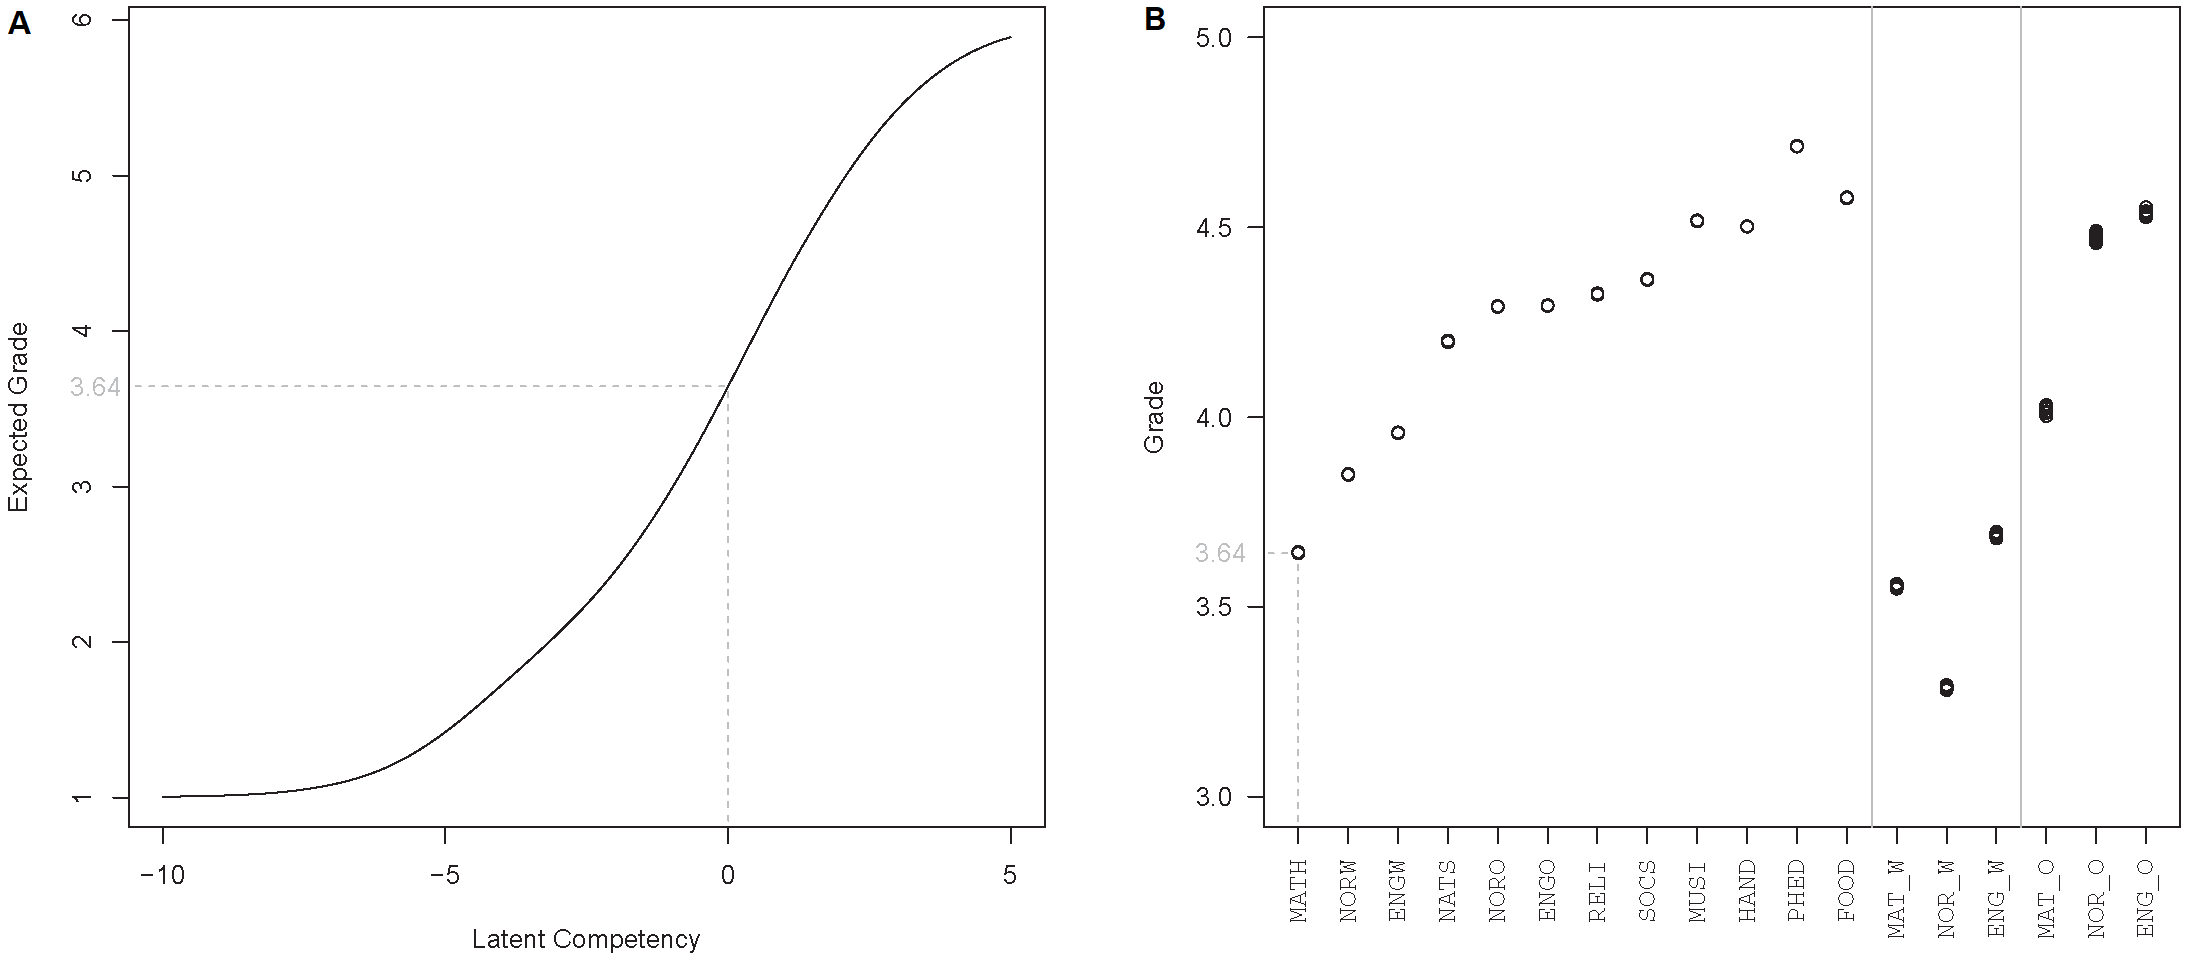
\includegraphics[width=1.5\textwidth]{./Figures/expected.png}
}{In Panel A, a median student evenly divides \textsc{math} candidates into 50\% below, and 50\% above him/her, whose $\theta$ is defined as zero. The expected grade of this median student 3.64 represents the \emph{overall difficulty} for \textsc{math}. Repeating this procedure for all 18 GPA subjects produces the scatter plot in Panel B. Subject with low expected grades such as \textsc{math} are more difficult while \textsc{phed} and \textsc{food} are easy subjects evidenced by the high expected grades from median students. Written- and oral-exams' overall difficulties are also shown. Results from ten imputed datasets were superimposed, leading to jitters in exam grades resultant from slightly larger imputation variations.}
